\chapter{Transportlag}

\section{Opgaveformulering}
I skal implementere en stop-and-wait protokol. Protokollen skal være pålidelig og skal anvende en 16 bit Internet-checksum til
fejldetektering. Det er et krav at protokollen skal kunne håndtere ødelagte data (f.eks. et forvansket frame pga. EMC). Det er ikke et absolut krav at protokollen skal kunne håndtere mistede data (timeout) men implementer timeout-funktionaliteten hvis tiden er til det - få stop-and-wait protokollen til at fungere først. Den maksimale længde af transportlagets data (payload) sættes til 1000 bytes. Dette lag skal overholde følgende segment header format:

\begin{figure}[htbp]
\centering
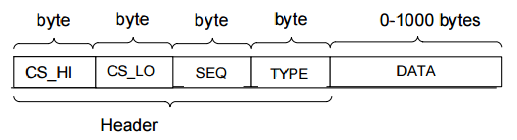
\includegraphics[width=1\linewidth]{Subpages/Billeder/Transportlag}
\caption{Transportlags protokol}
\label{fig:Transportlag}
\end{figure}

\textbf{CS\_HI:} Den mest betydende del af checksums-beregningen.\\
\textbf{CS\_LO:} Den mindst betydende del af checksums-beregningen.\\
\textbf{SEQ:} Sekvensnummer på den afsendte segment.\\
\textbf{TYPE:} 0 (DATA) 1 (ACK)\\
\textbf{DATA:} Payload på mellem 0-1000 bytes. Skal altid være af længden 0 ved ACK

